%!TEX root = ../Thesis.tex

\chapter{Metodología}\label{ch:chap5}

\epigraphhead[70]{
\epigraph{There was nowhere to go but everywhere, so just keep on rolling under the stars.}
{Jack Kerouac}}

A continuación se describe la metodología que se llevo a cabo para la tarea de \sd. 

Como ya se describió en el \autoref{ch:chap2} es necesaria una etapa de pre-procesamiento en el sistema; primero para eliminar de la señal de audio las cosas que no nos interesan (que en este caso son silencios), para lo que se usó un detector de energía y así ignorar los instantes en los que ningún interlocutor participa. 

Luego, también en la etapa de pre-procesamiento se encuentra el obtener vectores de características que representen de alguna manera la señal, y que sean mucho más fáciles de manipular. Para esta etapa se usaron los \ac{MFCC}, siguiendo el algoritmo \autoref{alg:mfcc}.  Después de obtener los vectores característicos, se agruparon mediante k-means++ (\autoref{alg:kmeanspp}) para de alguna forma discretizar todas las posibles palabras emitidas en el diálogo. Esta agrupación inicial nos permitirá reducir la dimensionalidad de los vectores, así como aglomerar aquellos que sean muy similares con respecto a los demás.

Después de esta etapa de clasificación, ya se tendrán los datos como observaciones que representarán las variables observadas del \ac{HMM}. Como se desconoce tal cual el número de personas involucradas en la grabación, se propondrán varios modelos $\mc{M}_d$ con $d$ estados ocultos. El valor de $d$ variará de acuerdo a qué tan extensas se deseen hacer las pruebas, pero a priori no hay un límite pre-establecido. 

Luego, corresponderá usar el algoritmo \ac{EM} con cada uno de los modelos $\mc{M}_d$ propuestos, tanto para estimar sus parámetros como para estimar su verosimilitud. Como ya se mencionó en \autoref{ch:chap4} esta etapa se realizará varias veces, para evitar el estancamiento del método y obtener un buen ajuste del modelo. Del modelo con mayor versomilitud se calculará la segmentación correspondiente, y se almacenará. 

Después, seguirá la etapa de selección de modelo. Se estimará \ac{BIC} para de todos los \ac{HMM} propuestos para generar una curva de selección. Como se verá en las pruebas, es necesario introducir un término de regularización en \ac{BIC} para que la penalización del modelo corresponda con las log-verosimilitudes obtenidas. 

Esto se puede hacer de la siguiente forma: 
\begin{equation}
BIC_{\lambda}(\mc{M}) = 2 \mc{L}_{max}(\mc{M}) - \lambda \cdot log N \cdot dim(M)
\end{equation}
aunque presenta el inconveniente de tener que encontrar el valor adecuado para $\lambda$ que penalice de buena forma los modelos. 

Para escoger el valor adecuado de $\lambda$ se realizará un análisis de sensibilidad, generando múltiples curvas de selección \ac{BIC} con diferentes valores de $\lambda$. Tanto la discretización como los rangos de $\lambda$ permitirán hacer una mejor búsqueda del parámetro. Con todas estas diferentes curvas, se tendrá una superficie, en donde en un eje variará el número de interlocutores del modelo, mientras que en el otro será el valor de regularización $\lambda$ el que cambiará. 

Se busca mediante este análisis encontrar la región de inflexión que divide a la superficie en dos: en la primera parte de la superficie, el valor de $\lambda$ será pequeño, por lo que siempre tendrán una mayor verosimilitud los modelos con más parámetros; mientras que en la segunda parte, la penalización sera muy grande, y se escogerán siempre los modelos más sencillos, sin darle tomar en cuenta su verosimilitud.

...

\section{Esquema general} 

El esquema general con las diferentes etapas que se realizan para estimar el número de personas así como su segmentación correspondiente.

\begin{figure}[bth]
  \centerline
  {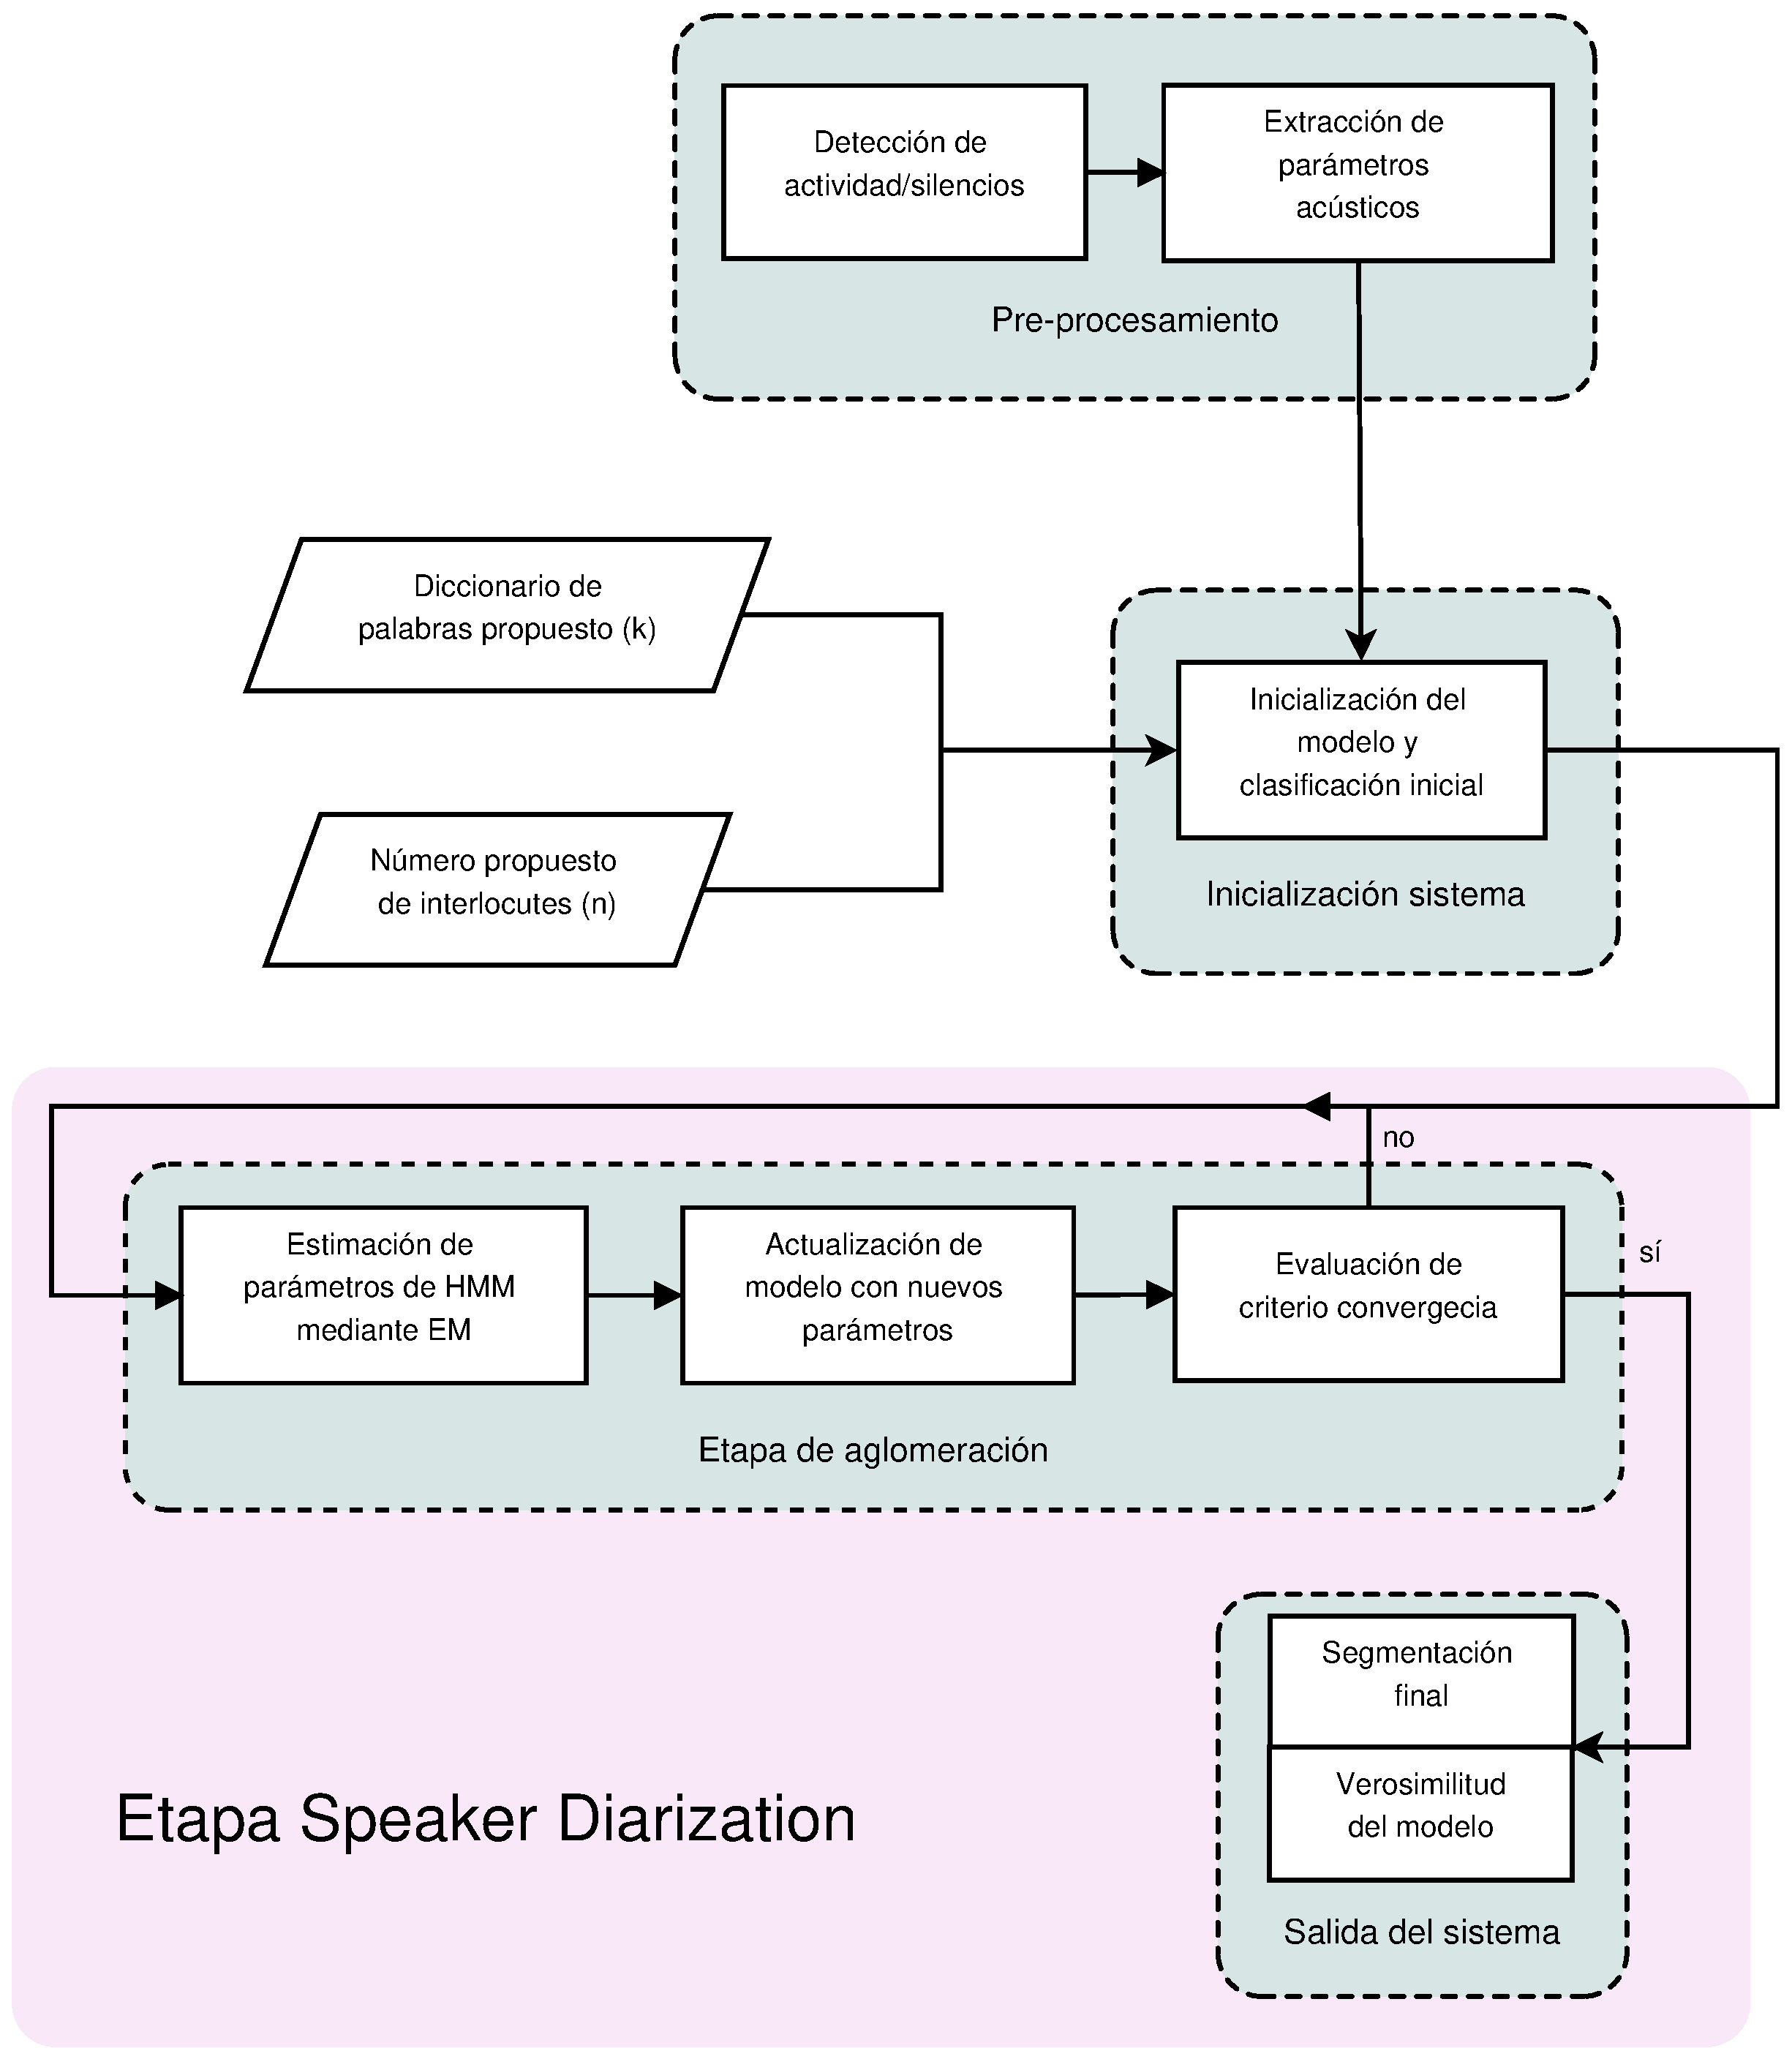
\includegraphics[width=1.5\linewidth]{gfx/chap5/general_flow}} \quad
  \caption{Esquema general.}
  \label{fig:esquema}
\end{figure}